\documentclass[12pt]{article}
\author{Alex Ho}
\title{FYS4150 - Computational Physics \\ Project 5}
\usepackage{listings}
\usepackage{graphicx}
\usepackage{verbatim}
\usepackage{amsmath}
\usepackage{float}
\usepackage[utf8]{inputenc}
\usepackage{xcolor}
\usepackage{booktabs}
\usepackage{hyperref}
\usepackage{placeins}
\usepackage{parskip}
\setlength\parskip{\baselineskip}
\setlength\parindent{0pt}

\lstset{
language=Python,
basicstyle=\ttfamily,
otherkeywords={self},             
keywordstyle=\ttfamily\color{blue!90!black},
keywords=[2]{True,False},
keywordstyle={[2]\ttfamily\color{blue!90!black}},
emph={MyClass,__init__},          
emphstyle=\ttfamily\color{red!80!black},    
stringstyle=\color{blue!90!black},
showstringspaces=false,
commentstyle=\color{blue!90!black},
breaklines=true,
tabsize=3,
moredelim=**[is][\color{blue}]{@}{@}
}
\begin{document}
\maketitle
\begin{abstract}
\end{abstract}
\newpage
\tableofcontents
\newpage
\section{Introduction} \label{section:intro}
In project 2, we studied the behaviour of two electrons interacting in a three dimensional harmonic oscillator potential. In that project, we had a look at the so called \emph{Eigenvalue problem} and used Jacobi's method to solve this problem. From that, we noted that Jacobi's method was not an optimal way to solve our quantum mechanical system, as it used a lot of CPU time to finish its calculations.

For this project, we will revisit this three dimensional harmonic oscillator with two electrons. This time, we will use a variational Monte Carlo method (VMC) method known as the Metropolis algorithm, which we also used in project 4, to solve this quantum mechanical system.

All relevant files used in this project can be found in the this GitHub page:
\url{https://github.com/AHo94/FYS3150_Projects/tree/master/Project5}
\section{Method} \label{section:method}
\subsection{Analytical form for the trial wave functions and local energies}
For this project, we will use natural units. That is $\hbar = c = e = m_e = 1$.
We will consider two electrons in a quantum dot with a frequency $\hbar \omega = 1$. The Hamiltonian for these two electrons is
\begin{align*}
H_0 = -\frac{1}{2}(\nabla_1^2 + \nabla_2^2) + \frac{1}{2}\omega^2(r_1^2 + r_2^2)
\end{align*}
The wave function for one electron in a harmonic oscillator potential is
\begin{align*}
\phi_{n_x, n_y, n_z}(x,y,z) = \frac{A}{2}H_{n_x}(\sqrt{\omega} x)H_{n_y}(\sqrt{\omega}y)H_{n_z}(\sqrt{\omega}z)e^{-\frac{\omega}{2}(x^2+y^2+z^2)}
\end{align*}
Where $H_{n_x}$ are Hermite polynomials and $A$ is a normalization constant. $n_x, n_y$ and $n_z$ are some quantum numbers. When the Hamiltonian is acted on this wave function, we obtain the energy. That is
\begin{align*}
H_0\phi_{n_x, n_y, n_z} &= \epsilon_{n_x, n_y, n_z}\phi_{n_x, n_y, n_z}
\end{align*}
with the energy given as
\begin{align*}
\epsilon_{n_x, n_y, n_z} &= \omega\left(n_x + n_y + n_z + \frac{3}{2} \right)
\end{align*}
For the ground state, $n_x = n_y = n_z = 0$, the energy of the single electron is
\begin{align*}
\epsilon_{0,0,0} = \frac{3}{2}\omega
\end{align*}
Let us now consider two electrons, so we have $\phi_{n_x, n_y, n_z}^1$ and $\phi_{n_x, n_y, n_z}^2$ (not squared!). Acting the Hamiltonian on both these wave functions gives
\begin{align*}
H_0(\phi_{n_x, n_y, n_z}^1 + \phi_{n_x, n_y, n_z}^2) &= \epsilon_{n_x, n_y, n_z}^1\phi_{n_x, n_y, n_z}^1 + \epsilon_{n_x, n_y, n_z}^2\phi_{n_x, n_y, n_z}^2 
\end{align*}
The total energy for these two electrons, when we consider the ground state, is then
\begin{align*}
\epsilon_{0,0,0}^{\text{tot}} &= \epsilon_{0,0,0}^1 + \epsilon_{0,0,0}^2 \\
&= \omega\left(\frac{3}{2} \right) + \omega\left(\frac{3}{2} \right)\\
&= 3\omega
\end{align*}

%% Add stuff for unperturbed case
The unperturbed wave function for the ground state of the two electron system is given as
\begin{align}
\Phi (\mathbf{r}_1, \mathbf{r}_2) = C\exp(-\omega(r_1^2 + r_2^2)/2)
\label{eq:Unpertubed_groundstate_wavefunc}
\end{align}
where $r_i = \sqrt{x_i^2 + y_i^2 + z_i^2}$. This wave function is symmetric when $r_1 \leftrightarrow -r_1$ and $r_2 \leftrightarrow -r_2$. Let us consider the trial wave function
\begin{align}
\psi_T(\mathbf{r}_1, \mathbf{r}_2) = \frac{1}{\sqrt{2}}\left(\psi_a(\mathbf{r}_1)\psi_b(\mathbf{r}_2)- \psi_a(\mathbf{r}_2)\psi_b(\mathbf{r}_1)  \right) 
\label{eq:Pauli-TrialFunc}
\end{align}
when we plug the wave function, given in \ref{eq:Unpertubed_groundstate_wavefunc}, into the trial Wave function in \ref{eq:Pauli-TrialFunc}, the result would be
\begin{align*}
\psi_T(\mathbf{r}_1, \mathbf{r}_2) = 0
\end{align*}
By Paulis principle, two electrons (or fermions) cannot be in same quantum state simultaneously. In order to allow such a trial wave function to exist, we will have to introduce spin statistics to the fermions. The fermions needs to be in different spin states if such a trial wave function is allowed to exist. The spin states an electron can be in is $s\pm 1/2$, and if our two electrons have different spins, the total spin of the system will therefore be zero.

Because of this, the Hamiltonian will not depend on the spin, and we can therefore drop the spin dependence. From this, we can use the ansatz that our first trial wave function can take the form 
\begin{align}
\psi_{T_1} &= C \exp\left(-\frac{\alpha \omega}{2}(r^2_1 + r^2_2)\right)
\label{eq:First_TrialFunc}
\end{align}
We can also make another ansatz, which gives us our second trial wave function
\begin{align}
\psi_{T_2} &= C \exp\left(-\frac{\alpha \omega}{2}(r^2_1 + r^2_2)\right)\exp\left(\frac{r_{12}}{2(1+\beta r_{12})}\right)
\label{eq:Second_TrialFunc}
\end{align}
where $r_{12} = \sqrt{r_1 - r_2}$ and $\alpha$ and $\beta$ are variational parameters. The second exponential in the $\psi_{T_2}$ is known as the Jastrow factor, which is there because it gives the lowest possible energy for the system, while reducing the amount of variational parameters.

Let us find the energy of the first trial function. First, we should rewrite the Hamiltonian in spherical coordinates. Our system does not depend on the radial coordinates, so the $\nabla$ operator, for electron $i$ in spherical coordinates, becomes
\begin{align*}
\nabla^2_i = -\frac{1}{2} \frac{d^2}{dr^2_i} - \frac{1}{r_i}\frac{d}{dr_i}
\end{align*}
By acting the Hamiltonian on $\psi_{T_1}$, we get
\begin{align*}
H_0\psi_{T_1} = \left(-\frac{d^2}{dr^2_1} - \frac{1}{r_1}\frac{d}{dr_1} -\frac{d^2}{dr^2_2} - \frac{1}{r_2}\frac{d}{dr_2} + \frac{1}{2}\omega(r_1^2+r_2^2)\right)\psi_{T_1}
\end{align*}
There will be a lot of derivatives to keep track of here, so I will take this step by step. Let us first differentiate with respect to $r_1$ first. The first derivative is
\begin{align*}
\frac{d}{dr_1}\exp\left(-\frac{\alpha \omega}{2}(r^2_1 + r^2_2)\right) &= \left( -\alpha \omega r_1 \right)\exp\left(-\frac{\alpha \omega}{2}(r^2_1 + r^2_2)\right) \\
&= -\alpha \omega r_1 \psi_{T_1}
\end{align*}
The second derivative then becomes
\begin{align*}
\frac{d^2}{dr_1^2}\exp\left(-\frac{\alpha \omega}{2}(r^2_1 + r^2_2)\right) &= \frac{d}{dr_1}\left[-\alpha \omega r_1 \exp\left(-\frac{\alpha \omega}{2}(r^2_1 + r^2_2)\right)\right]\\
&= (-\alpha \omega + \alpha^2 \omega^2 r_1^2)\exp\left(-\frac{\alpha \omega}{2}(r^2_1 + r^2_2)\right) \\
&= (\alpha^2 \omega^2 r_1^2 - \alpha \omega)\psi_{T_1}
\end{align*}
In short, the kinetic term is
\begin{align}
\nabla_1^2 \psi_{T_1} =-\frac{1}{2}(\alpha^2\omega^2r_1^2 -3 \alpha \omega)\psi_{T_1}
\label{eq:Kinetic_psi1}
\end{align}
I will skip the calculation for the derivative with respect to $r_2$, but the results are
\begin{align*}
\frac{d}{dr_2}\psi_{T_1} &=  -\alpha \omega r_2 \psi_{T_1} \\
\frac{d^2}{dr_2^2}\psi_{T_1} &= (\alpha^2 \omega^2 r_2^2 - \alpha \omega)\psi_{T_1}
\end{align*}
which gives
\begin{align*}
\nabla_1^2 \psi_{T_1} =-\frac{1}{2}(\alpha^2\omega^2r_2^2 -3 \alpha \omega)\psi_{T_1}
\end{align*}
The local energy, for this trial function, is then
\begin{align}
E_{L_1} &= -\frac{1}{2} (\alpha^2 \omega^2 r_1^2 - 3\alpha \omega)  - \frac{1}{2} (\alpha^2 \omega^2 r_2^2 - 3\alpha \omega) + \frac{1}{2}\omega^2(r_1^2 + r_2^2) \nonumber \\
&= 3 \alpha \omega  - \frac{1}{2}\alpha^2 \omega^2 (r_1^2 + r_2^2) + \frac{1}{2}\omega(r_1^2 + r_2^2) \nonumber \\
&= 3\alpha \omega + \frac{1}{2}(\omega^2 - \alpha^2 \omega^2)(r_1^2 + r_2^2) \nonumber \\
&= 3 \alpha \omega +  \frac{1}{2}\omega^2(1-\alpha^2)(r_1^2 + r_2^2)
\label{eq:Energy_T1}
\end{align}
which is exactly what we wanted to show. We will skip the derivation of the analytical local energy for the second trial wave function. If we add Coulomb interaction, the Hamiltonian now becomes
\begin{align*}
H_0 = \displaystyle \sum_{i=1}^N\left(-\frac{1}{2}\nabla_i^2 + \frac{1}{2}\omega^2r_i^2 \right) + \sum_{i<j}\frac{1}{r_{ij}}
\end{align*}
and the local energy for the first trial wave function is then
\begin{align}
E_{L1} = 3 \alpha \omega +  \frac{1}{2}\omega^2(1-\alpha^2)(r_1^2 + r_2^2) + \frac{1}{r_{12}}
\label{eq:Energy_T1_Coulomb}
\end{align}
where $r_{12}= |\mathbf{r}_1 - \mathbf{r}_2|$. The analytical expression for the second trial wave function, with Coulomb interaction, is then
\begin{align}
E_{L2} = E_{L1} + \frac{1}{2(1+\beta r_{12})^2}\left[\alpha \omega r_{12} - \frac{1}{2(1+\beta r_{12})} - \frac{2}{r_{12}} + \frac{2\beta}{1+\beta r_{12}} \right]
\label{eq:Energy_T2_Coulomb}
\end{align}
with $E_{L1}$ given in equation \ref{eq:Energy_T1_Coulomb}.

\subsection{The Metropolis Algorithm}
We will once again, like in project 4, use the Metropolis algorithm to solve our quantum mechanical system. The algorithm is as follows: for every Monte Carlo cycle we 
\begin{itemize}
\item \textbf{1)} Start the electrons at an arbitrary position. We let the electron start at the position $x,y,z \in [-1,1]$, which we get from a normal distribution.

\item \textbf{2)} Give the electrons a new position determined by $\mathbf{R}' = \mathbf{R} + \delta\times s$, where $\mathbf{R} = (\mathbf{r}_1, \mathbf{r}_2, ..., \mathbf{r}_N)$, $s$ is a random number generated from a normal distribution such that $s\in [-1,1]$ and $\delta$ is a small step length. Note that $\delta \times r$ is different for every component, e.g
\begin{align*}
\mathbf{r_1}' = (x_1 + \delta\times s_1, y_1 + \delta\times s_2, z_1 + \delta\times s_3)
\end{align*} For this project we will consider $N=2$ electrons.

\item \textbf{3)} Calculate $w = P(\mathbf{R}')/P(\mathbf{R}) = |\Psi(\mathbf{R}')|^2/|\Psi(\mathbf{R})|^2$, where $\Psi$ is the wave function we will consider (i.e the trial wave functions $\psi_{T1}$ and $\psi_{T2}$ mentioned previously). Pick a random number $p\in [0,1]$, also given from a normal distribution function. We now have to consider these two cases

\item \textbf{Case 1}: If $p <= w$, we accept this new position change and use the calculated $\mathbf{R}'$ to calculate the local energy. The system has now reached a lower energy state.

\item \textbf{Case 2}: If $p > w$, we do not accept this new position and use the old position $\mathbf{R}$ to calculate the local energy.

\item \textbf{4)} Use the new or old position (depending on whatever case above hits) to calculate the local energy $E_L = \frac{1}{\Psi} H_0\Psi$. 
\end{itemize}
By calculating the fraction $|\Psi(\mathbf{R}')|^2/|\Psi(\mathbf{R})|^2$, we eliminate the requirement to compute the integral given in
\begin{align*}
P(\mathbf{R}) = \frac{|\Psi(\mathbf{R})|^2}{\int |\Psi(\mathbf{R})|^2 d\mathbf{R}}
\end{align*}
which is similar to what we did in project 4. In project 4, by calculating $p<= e^{-\beta \delta E}$, we could skip the calculation of the partition function $Z$. 

Once again, by running this for $N_{mc}$ Monte Carlo cycles, we find the energy expectation value as
\begin{align*}
\langle E \rangle = \displaystyle \frac{1}{N_{mc}}\sum_i E_i
\end{align*}
where $E_i$ is all the energy samples calculated from the Metropolis algorithm. One can also find the expectation value of the mean distance at the energy minimum $r_{12} = |\mathbf{r}_1 - \mathbf{r}_2|$ in the same way.

One of the main advantages of using variational Monte Carlo methods is that we can carry out our calculations using cartesian coordinates. If we look back to project 2, we had to define new variables in order to solve the eigenvalue problem.

\subsection{Algorithm that determines the step length}
We would like to find an algorithm that, for a given value of $\alpha$, uses an optimal value of the step length $\delta$. This should ideally result to roughly 50\% accepted moves in the metropolis algorithm. One can run the program multiple times to determine the step length. However, one can also find an analytical solution, which would automatize the optimal step length.

Since we are looking at accepted moves, we will take a look at the equation
\begin{align*}
p = \frac{|\Psi(\mathbf{R'})|^2}{|\Psi(\mathbf{R})|^2}
\end{align*}
which was used to determine whether we accept a move or not in the Metropolis algorithm. The length $|\mathbf{r}_1'| = \mathbf{r}_1 + \delta \times s = r_1'$ is now
\begin{align*}
r_1' = \sqrt{(x_1 + \delta s_1)^2 + (y_1 + \delta s_2)^2 + (z_1 + \delta s_3)^2}
\end{align*} We let $p = 0.5$, as we want roughly 50\% accepted moves. We then plug in the first trial wave function to determine an optimal $\delta$ for a given $\alpha$, which gives
\begin{align*}
0.5 &= \frac{1}{\exp\left[-\alpha \omega(r_1^2+r_2^2) \right]} \big(\exp\big[-\alpha \omega \big((x_1 + \delta s_1)^2 + (y_1 + \delta s_2)^2  \\
& + (z_1 + \delta s_3)^2 + (x_2 + \delta s_4)^2 + (y_2 + \delta s_5)^2 + (z_2 + \delta s_6)^2\big)\big]\big) \\
&= \frac{1}{\exp[-\alpha \omega (r_1^2 + r_2^2)]}\big(\exp[-\alpha \omega\big(x_1^2 + y_1^2 + z_1^2 + 2\delta(x_1s_1 + y_1s_2 + z_1s_3) + \\
& x_2^2 + y_2^2 + z_2^2 + 2\delta(x_2s_4 + y_2s_5 + z_2 s_6) +\delta^2(s_1^2 + s_2^2 + s_3^2 + s_4^2 + s_5^2 + s_6^2) \big)]  \big) \\
&= \exp\big[-\alpha \omega\big(2\delta(x_1s_1 + y_1s_2 + z _1s_3 + x_2s_4 + y_2s_5 + z_2 s_6) \\
& +\delta^2(s_1^2 + s_2^2 + s_3^2 + s_4^2 + s_5^2 + s_6^2) \big) \big]
\end{align*}
where we have in the last line used  $x^2 + y^2 + z^2 = r^2$ for both $r_1$ and $r_2$, thus cancelling the denominator. Taking the logarithm on both sides gives
\begin{align*}
\ln(0.5) &= -\alpha \omega\big(2\delta(x_1s_1 + y_1s_2 + z _1s_3 + x_2s_4 + y_2s_5 + z_2 s_6) \\
& +\delta^2(s_1^2 + s_2^2 + s_3^2 + s_4^2 + s_5^2 + s_6^2) \big) \\
\implies & a\delta^2 + b\delta + c = 0
\end{align*}
where we have defined
\begin{align*}
a &= s_1^2 + s_2^2 + s_3^2 + s_4^2 + s_5^2 + s_6^2 \\
b &= 2(x_1s_1 + y_1s_2 + z _1s_3 + x_2s_4 + y_2s_5 + z_2 s_6) \\
c &= \frac{\ln(0.5)}{\alpha \omega}
\end{align*}
This is just a second order equation for $\delta$. We require that $\delta$ is always positive, so when we solve this equation for $\delta$, we will have to only consider the positive part. Doing this results to
\begin{align}
\delta = \frac{1}{2a}(-b + \sqrt{b^2 - 4ac})
\label{eq:step_length_algo}
\end{align}
Implementing this in the program \emph{should} ideally result to roughly 50\% of the configurations being accepted. However, this will not be the case. We will see that the the number of accepted configurations will float around 65\% for most cases. This is a little far away from the 50\% we wanted, but it should suffice.

\subsection{Results from project 2}
It is a good idea to note down some relations from project 2, since we will compare a lot of our results with that project. Previously, we found that an electron in a harmonic oscillator potential had the energy
\begin{align*}
E_{nl} = \hbar \omega \left(2n + l + \frac{3}{2} \right)
\end{align*}
Using natural units we have $\hbar = 1$. We also neglect the angular movements, so $l = 0$ and in the ground state, we let the quantum number $n=0$. This energy does not take into account center of mass energy $E_{cm}$. Because of this, we will have to add $E_{cm} = 1.5$ to $E_{nl}$ when we compare our results.
\section{Implementation} \label{section:implement}
Like in the previous projects, I will do all the calculations in C++ and plot the results in Python.

For this project, I have object oriented the whole program. The class\\ \texttt{Wavefunctions} initializes a so called \emph{functor}. The idea here is to create the wave functions as an object that acts as a (c++) function. This will make the program a lot more flexible, as we can choose whether we want to use the first or the second trial wave function.

I have also made a class called \texttt{Metropolis\_quantum}. This class contains three different Metropolis solving functions. The first one uses the local energy $E_{L1}$ in the calculation, the second uses the local energy $E_{L2}$ and the final one is made specifically to test the virial problem.

I have also used the class \texttt{vec3}, which we developed in project 3. This class will make it easier to keep track of all the components contained within the radius variable $\mathbf{r} = (x, y, z)$, as it contains methods to do certain vector calculations, e.g finding vector length and vector addition. 


\subsection{Testing the Metropolis algorithm}
Before we proceed with the results, we should check if the Metropolis algorithm works as it should. When calculating the local energy, we should use a numerical approach to calculate the kinetic term $\nabla^2\psi$. However, we already have the analytical expression of the local energy $E_{L1}$, given in equation \ref{eq:Energy_T1}. From that, we also know which terms contributes to the kinetic energy. In fact, the kinetic energy is given in equation \ref{eq:Kinetic_psi1}, which we can use to test the Metropolis algorithm.

By implementing this term as its own function \texttt{LaplaceAnalytic}, we run the program with the analytical kinetic energy. Using $10^6$ Monte Carlo cycles, $\alpha = 1$, $\omega = 1$ and no Coulomb interaction, the result is:
\begin{lstlisting}
@Monte Monte Carlo cycles = 1000000
Kinetic numeric = 3
Variance = 0
Accepted configs (percentage) = 0.62867
Time elapsed: 1.576s@
\end{lstlisting}
So the numerical energy, using the analytical expression of the kinetic energy, is exactly 3! The variance is exactly zero as well, which is what we would expect from this test. Also note the number of accepted configurations. The algorithm for an optimal step length, given in equation \ref{eq:step_length_algo}, gives roughly 63\% accepted configurations. Not exactly perfect, but good enough.

We can now also test, with the same values of $\alpha$ and $\omega$, if the numerical derivation of the kinetic term works. The discretized numerical second derivative is given as
\begin{align*}
\left(\frac{d^2f}{dx^2}\right) = \frac{f(x + \Delta x) + f(x - \Delta x) - 2f(x)}{\Delta x^2}
\end{align*}
The Laplace operator for all three dimensions is thus
\begin{align*}
\nabla^2 f = \displaystyle \sum_{i=1}^3 \frac{f(x_i + \Delta x) + f(x_i - \Delta x) - 2f(x_i)}{\Delta x^2} 
\end{align*}
where $i=1,2,3$ corresponds to the $x,y,z$ components and $\Delta x$ is the same for every direction. We let $\Delta x = 10^{-5}$ and running this for the first trial function gives
\begin{lstlisting}
@Monte Monte Carlo cycles = 1000000
Kinetic numeric = 3
Variance = 3.30573e-011
Accepted configs (percentage) = 0.628217
Time elapsed: 10.504s@
\end{lstlisting}
The result is incredibly good. The energy is (almost) exactly 3 and the variance is very close to zero as well. We can therefore calculate the kinetic term of the local energy by using numerical derivation for any wave function.

However, we should also note down the time it took for the Metropolis algorithm to compute the energy expectation value. The Metropolis algorithm was almost 10 times faster if were were to use the exact analytical expression of the kinetic term instead of calculating it numerically. Because of this, we will use the analytical expressions of the local energies to save CPU time. Also, we should really appreciate the computation speed of the Metropolis algorithm. If we look back to project 2, the Jacobi's method often times used more than  5 minutes to calculate the energies.

\section{Results}\label{section:results}
\subsection{The first trial wave function}
We will first consider the first trial wave function given in \ref{eq:First_TrialFunc}. 
\subsubsection{Finding the optimal $\alpha$}
Let us now plot the energy (expectation value) and variance as a function of of the variational parameter $\alpha$. We can use these determine the optimal value of $\alpha$, which we can use to compare with our results from project 2. One thing to note is that the optimal variational parameter may be different for different frequencies $\omega$.

Plots of the energy and variance, as a function of $\alpha$, using $\omega = 1$, can be found in figure \ref{fig:Energy_alpha_omega1} and \ref{fig:Variance_alpha_omega1} respectively. We can see that both of them has a minimum, but oddly enough at different values of $\alpha$. We would expect that the energy should be at its minimum when $\alpha = 1$ or smaller. However, the plot in figure \ref{fig:Energy_alpha_omega1} says that it is not quite the case. The minimum is shifted to a slightly larger $\alpha$ value, where the minimum is now at $\alpha = 1.08$.

However, if we look at the plot of variance in \ref{fig:Variance_alpha_omega1}, we see that the minimum is at $\alpha = 1$. Also note that the variance here is exactly zero, which also means that the standard deviation is also zero. Because of this, the calculated energy at $\alpha = 1$ is exact, i.e there are no errors here. On the other hand, if we look at table \ref{table:AlphaMinimum_omega1} \footnote{Full data set, for this case, can be found at \url{https://github.com/AHo94/FYS3150_Projects/blob/master/Project5/build-Project5_cpp_program-Desktop_Qt_5_7_0_MinGW_32bit-Release/Energy_Alpha_Mdistance_omega_1.00.txt}}, the calculated minimum at $\alpha=1.08$ has a variance of $\sigma_E^2 = 0.0196079$, or $\sigma_E = 0.14002$, which means that the calculated energy at $\alpha = 1.08$ has a small margin of error which also means that it may not actually be the minimum. We can therefore safely say that the optimal value of the variational parameter, using the first trial wave function at $\omega = 1$ is $\alpha = 1$.

\begin{figure}[h]
\centering
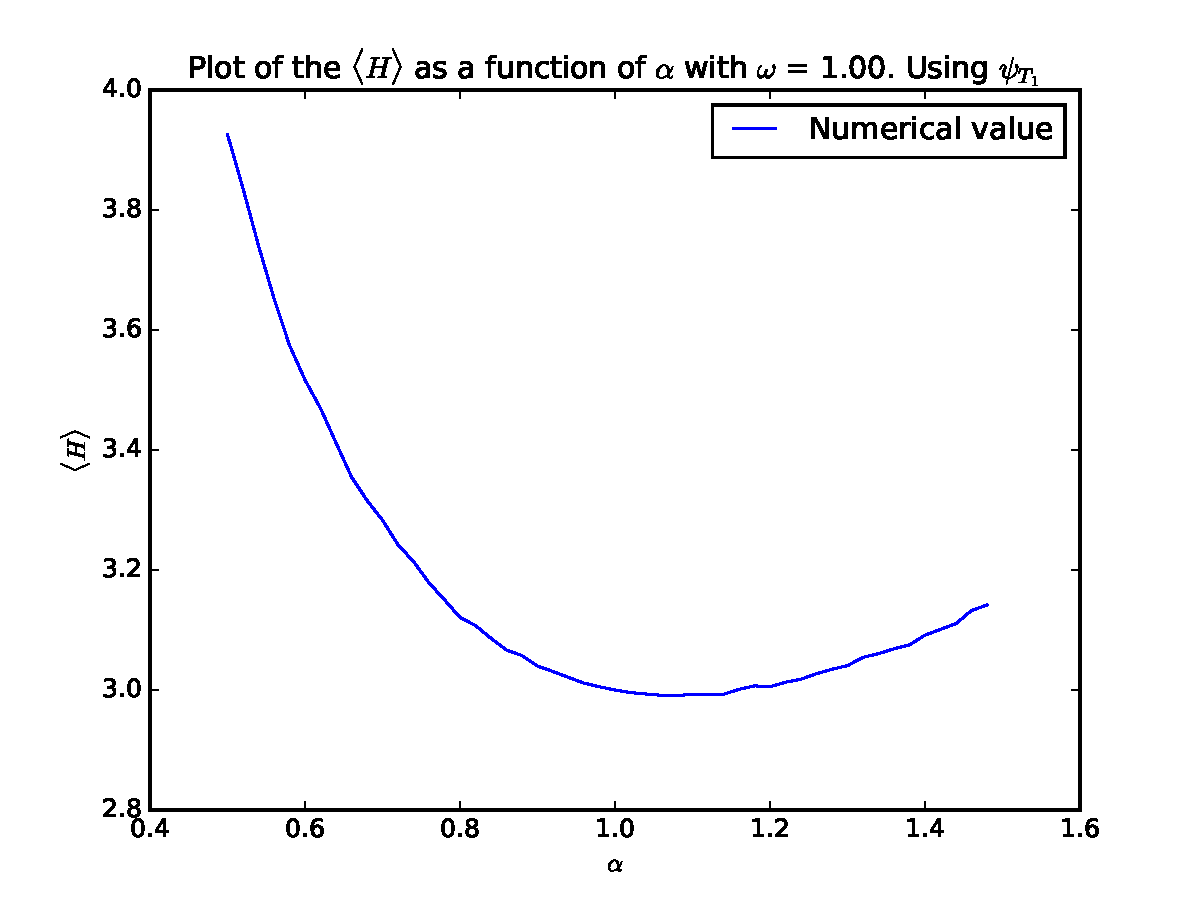
\includegraphics[width=\linewidth]{Plots/Energy_alpha_plot_omega1.pdf}
\caption{Plot of the Energy as a function of $\alpha$ with $\omega = 1$.}
\label{fig:Energy_alpha_omega1}
\end{figure}
\begin{figure}[h]
\centering
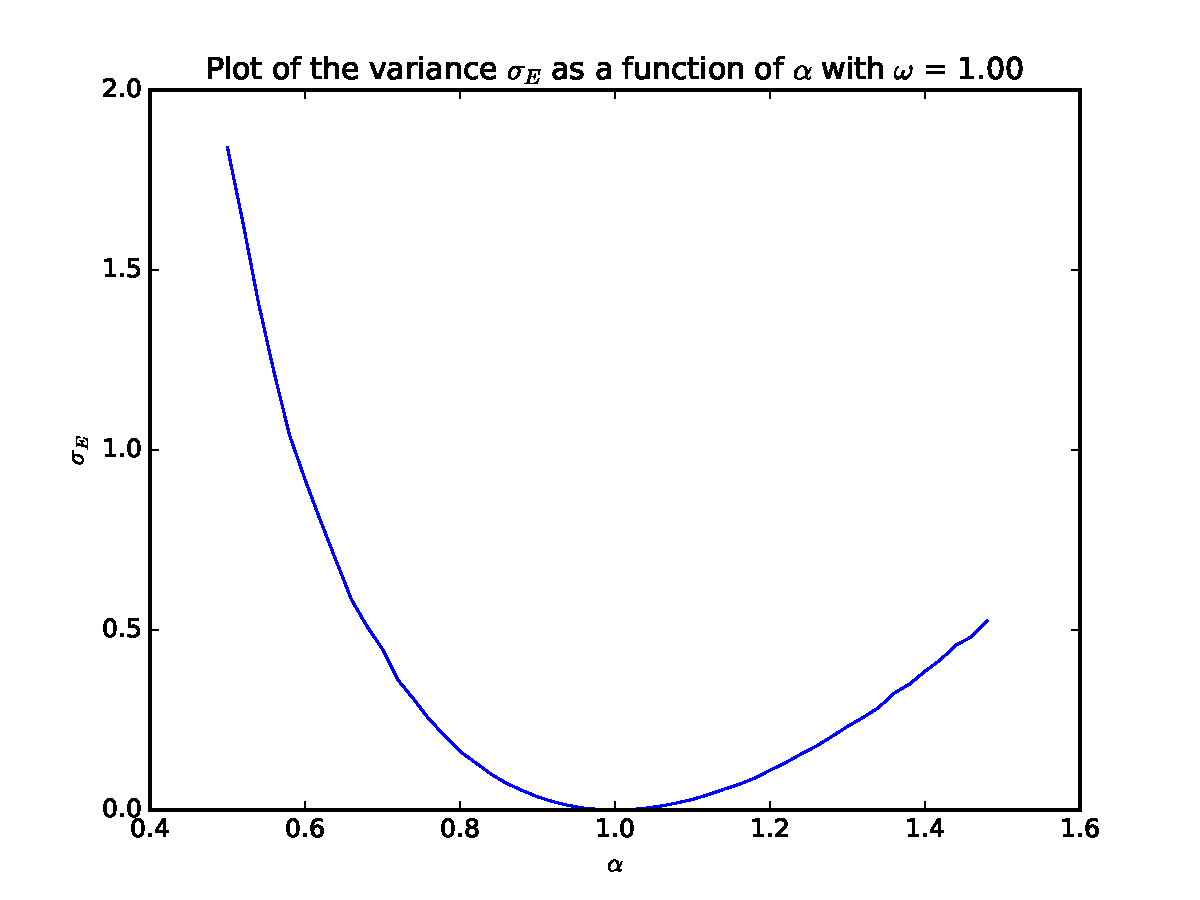
\includegraphics[width=\linewidth]{Plots/Variance_alpha_plot_omega1.pdf}
\caption{Plot of the variance as a function of $\alpha$ with $\omega = 1$.}
\label{fig:Variance_alpha_omega1}
\end{figure}

\begin{table}
\begin{center}
	\begin{tabular}{| l | l | l |}
	\hline 
	$\alpha$ & Energy & Variance \\ \hline
	0.98 & 3.00541 & 0.0013228 \\
	1 & 3 & 0 \\
	1.02 & 2.9957 & 0.00130505 \\
	1.04 & 2.99328 & 0.00504903 \\
	1.06 & 2.99118 & 0.0112062 \\
	1.08 & 2.99027 & 0.0196079 \\
	1.1 & 2.99322 & 0.0293394 \\
	1.12 & 2.99256 & 0.0423141 \\
	1.14 & 2.99289 & 0.0572603 \\
	1.16 & 3.00114 & 0.0713725 \\ \hline
	\end{tabular}
\caption{The energy, variance and $\alpha$ values near the minimum point.}
\label{table:AlphaMinimum_omega1}
\end{center}
\end{table}
We obtain similar results for the cases with $\omega = 0.5$ and $\omega = 0.01$. The energy, for both cases, are also not at its minimum when $\alpha = 1$, but shifted to a slightly larger $\alpha$ value. However, the variance is once again zero (almost zero for $\omega = 0.01$) when $\alpha = 1$, so we can also safely say that the optimal variational parameter is $\alpha = 1$ for both cases. The plots of these can be found in the appendix.

One might wonder, how stable is the Metropolis algorithm? We know that the results are better when we increase the number of Monte Carlo cycles. However, this is not exactly the case for the first trial wave function when we use the analytical local energy. If we run our previous tests with different Monte Carlo cycles, we will see that our algorithm is very, very stable, even for lower number of Monte Carlo cycles.

An example of this can be found in figure \ref{fig:Stability_1}, with $\omega = 1$. As we see, even with lower number of Monte Carlo cycles, the results are incredibly stable. It should, again, be noted that we have used the analytic local energy in the calculations, which may be the reason for such a stable results. However, we will see later, when we test the virial problem, that lower number of Monte Carlo cycles will give less table/exact results. \footnote{We were asked to plot the stability as a function of Monte Carlo cycles. However, I was not sure what to plot, as the computed of the energies were exactly the same for every Monte Carlo cycle.}
\begin{figure}[h]
\centering
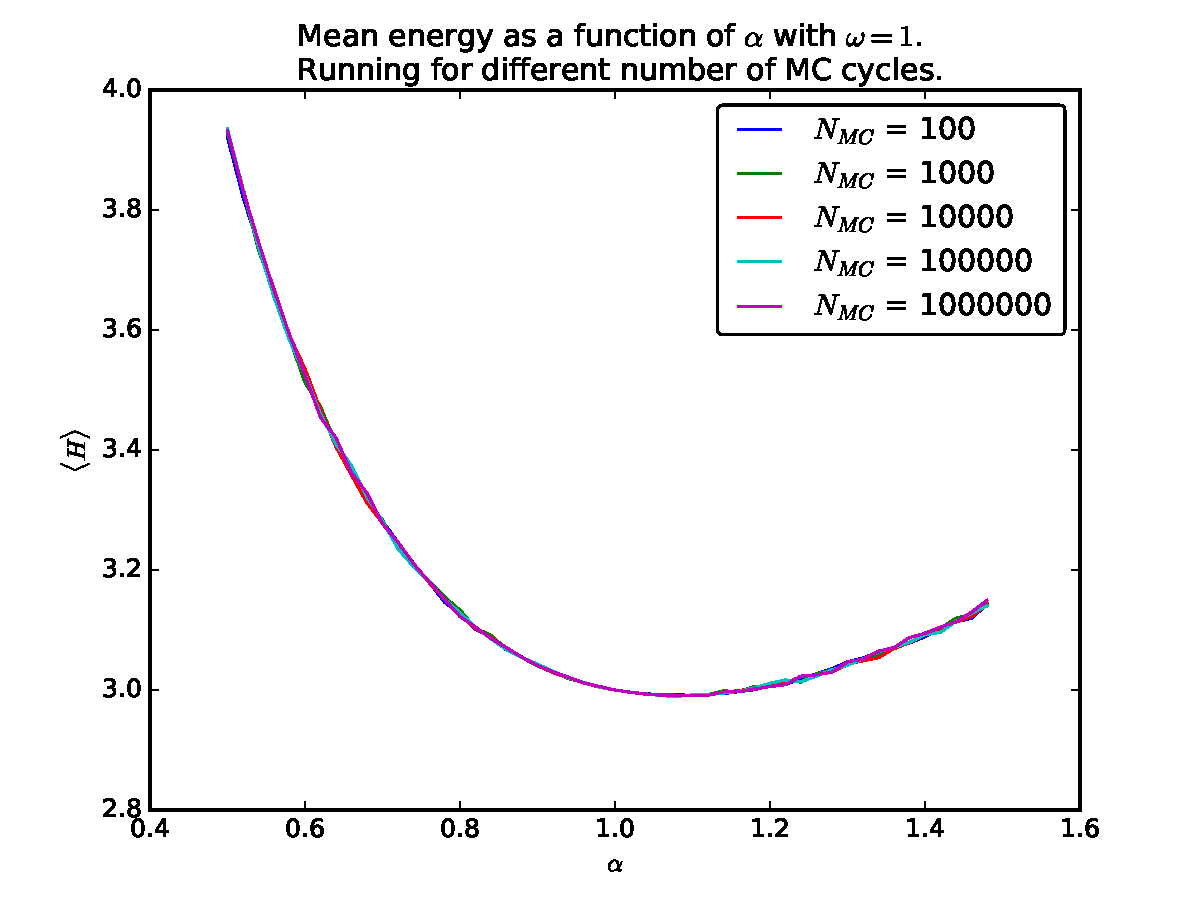
\includegraphics[width=\linewidth]{Plots/Stability_check.pdf}
\caption{Example of the stability of the Metropolis algorithm.}
\label{fig:Stability_1}
\end{figure}

\FloatBarrier
\subsubsection{The mean distance}
Now that we have found the optimal variational parameter, we can use it to calculate the mean distance $r_{12}$ between the two electrons at the energy minimum. Using the frequency values $\omega = 0.01, 0.5, 1$, the calculated mean distance  can be found in table \ref{table:Mean_Distance}.
\begin{table}
\begin{center}
	\begin{tabular}{| l | c |}
	\hline 
	$\omega$ & Mean distance \\ \hline
	1 & 1.55877 \\ 
	0.5 & 2.34729 \\
	0.01 & 16.5251 \\ \hline
	\end{tabular}
\caption{The mean distance of between the electrons for different frequencies, using the first trial wave function $\psi_{T_1}$.}
\label{table:Mean_Distance}
\end{center}
\end{table}

Let us quickly go back to project 2, where we used the analogy where two electrons are bound by a spring. The electrons now oscillate back and forth due to the oscillation of the spring. 

For smaller frequencies, we can imagine that the spring is not very stiff, which means that the electrons can be drawn further apart before they get pulled back in by the spring. Because they can be further apart, the average distance between these two electrons will therefore be larger, which is exactly what we see from the computed results above.

For larger frequencies, we imagine that the spring is a lot stiffer, so the electrons cannot be drawn as far apart. The average distance is thus smaller when we have larger frequencies. This also agrees with the computed value above. 

The results of the mean distance gives the same physical interpretation as the one from project 2 of our three dimensional harmonic oscillator. The difference here is that we use the Metropolis algorithm in this project, whereas we used the Jacobi's method in project 2. So far, we have seen that the former is a lot faster than the latter algorithm.

Let us also have a look at the number of accepted configurations for every $\alpha$ value we computed. From the previous section, we noted that the algorithm that is used to determine an optimal step length $\delta$ resulted to roughly 60 \% accepted configurations. Ideally, we would like to have 50\% accepted configurations, but 60\% should be good enough. Figure \ref{fig:AcceptedConfigs} shows a plot of the number of accepted configurations (percentage of the total number of Monte Carlo cycles) as a function of $\alpha$. We see that the number of accepted configurations is roughly 62.7\%  for every frequency.

\begin{figure}[h]
\centering
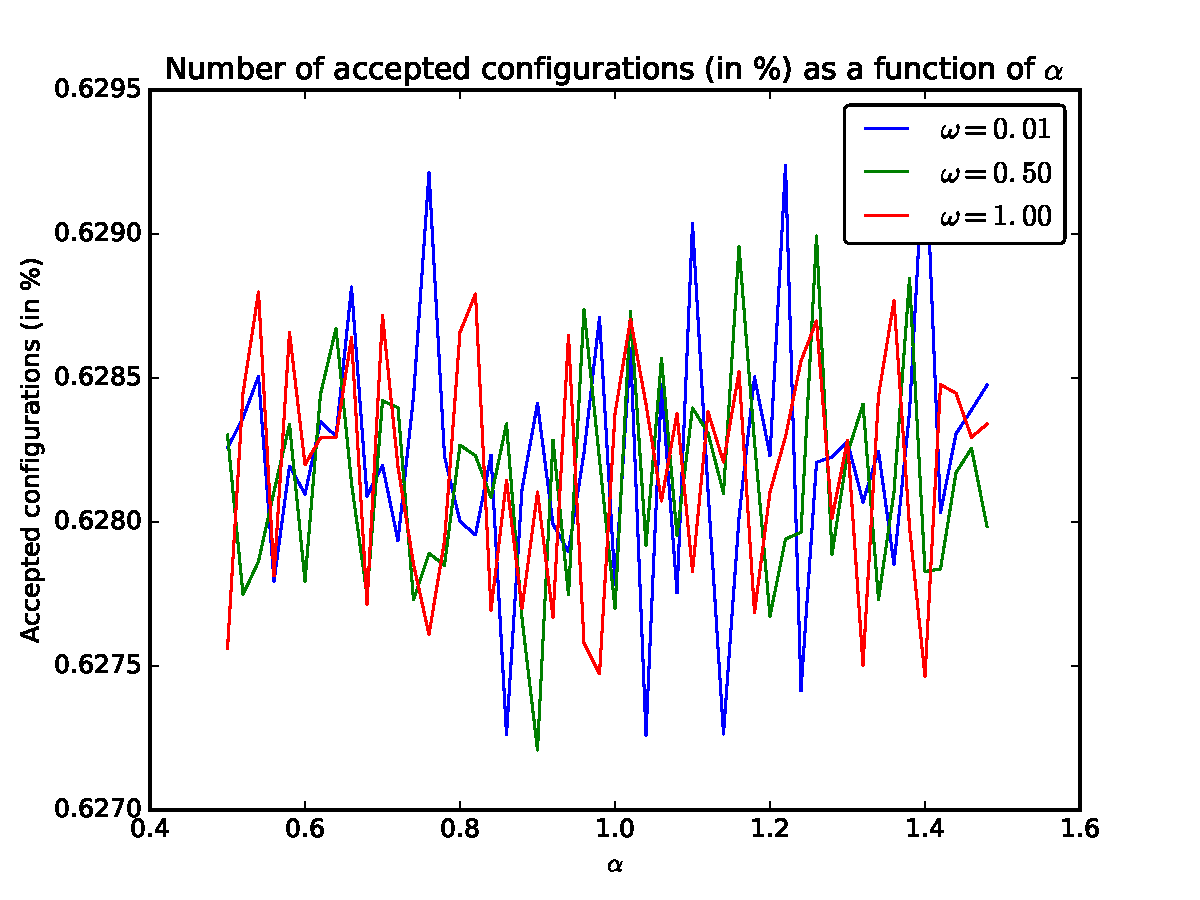
\includegraphics[width=\linewidth]{Plots/AcceptedConfigs.pdf}
\caption{Number of accepted confugrations for each different Metropolis run. The number of accepted configurations is in percentage of the total number of Monte Carlo cycles.}
\label{fig:AcceptedConfigs}
\end{figure}

  
\FloatBarrier
\subsection{The second trial wave function}
\subsubsection{Finding the optimal variational parameters}
We will now consider the second trial wave function given in  \ref{eq:Second_TrialFunc}. Let us first find the optimal variational parameters of both $\alpha$ and $\beta$. To do so, we can simply run the Metropolis algorithm as a for loop of different $\alpha$ and $\beta$ values. It should, again, be noted that the optimal parameters may be different for different frequencies.

Running this for different values of $\alpha$ and $\beta$ gives a lot of data in the output file. I have therefore used Python to find the optimal value of both the variational parameters. The strategy is to find the energy minimum in the array of energies. With the energy minimum, we can find which array element that corresponds to this energy minimum. Once we have the array element index, we can use that to find the corresponding $\alpha$ and $\beta$ values in their respective arrays.

The output below shows the optimal values of $\alpha$ and $\beta$, as well as the lowest energy and the standard deviation, when we do our calculation. These values were obtained when we ran with $10^6$ Monte Carlo cycles. The variational parameters will then be manually set back into C++ to do the remaining tasks. Table \ref{table:Optimal_AlphaBeta} shows the optimal $\alpha$ and $\beta$ values that we got from the output below.
\begin{lstlisting}
@For omega =  1.0
Lowest energy =  3.72737
Optimal Alpha value =  0.98
Optimal Beta value =  0.52
Standard deviation =  0.112554875505

For omega =  0.5
Lowest energy =  1.99883
Optimal Alpha value =  0.98
Optimal Beta value =  0.36
Standard deviation =  0.0721291203329

For omega =  0.01
Lowest energy =  0.0859782
Optimal Alpha value =  0.6
Optimal Beta value =  0.2
Standard deviation =  0.0171850807388@
\end{lstlisting}

\begin{table}
\begin{center}
	\begin{tabular}{| l | l | l |}
	\hline
	 $\omega$ & $\alpha$ & $\beta$ \\ \hline
	 0.01 & 0.6 & 0.2 \\
	 0.5 & 0.98 & 0.36 \\
	 1 & 0.98 & 0.52 \\ \hline
	\end{tabular}
\caption{Optimal values of $\alpha$ and $\beta$ for the different frequencies.}
\label{table:Optimal_AlphaBeta}
\end{center}
\end{table}

We can also plot how the energy evolves as we change the variational parameters. I will only plot the one for $\omega = 1$, as the other frequencies will give similar results. The plot can be found in \ref{fig:3DPlot_AlphaBeta_Optimal}.  One may think, when looking at the plot, that we have not quite reached the minimum energy. However, I have tested this multiple times for different ranges of $\alpha$ and $\beta$, and I can safely say that there is a minimum in that plot.
\begin{figure}[h]
\centering
%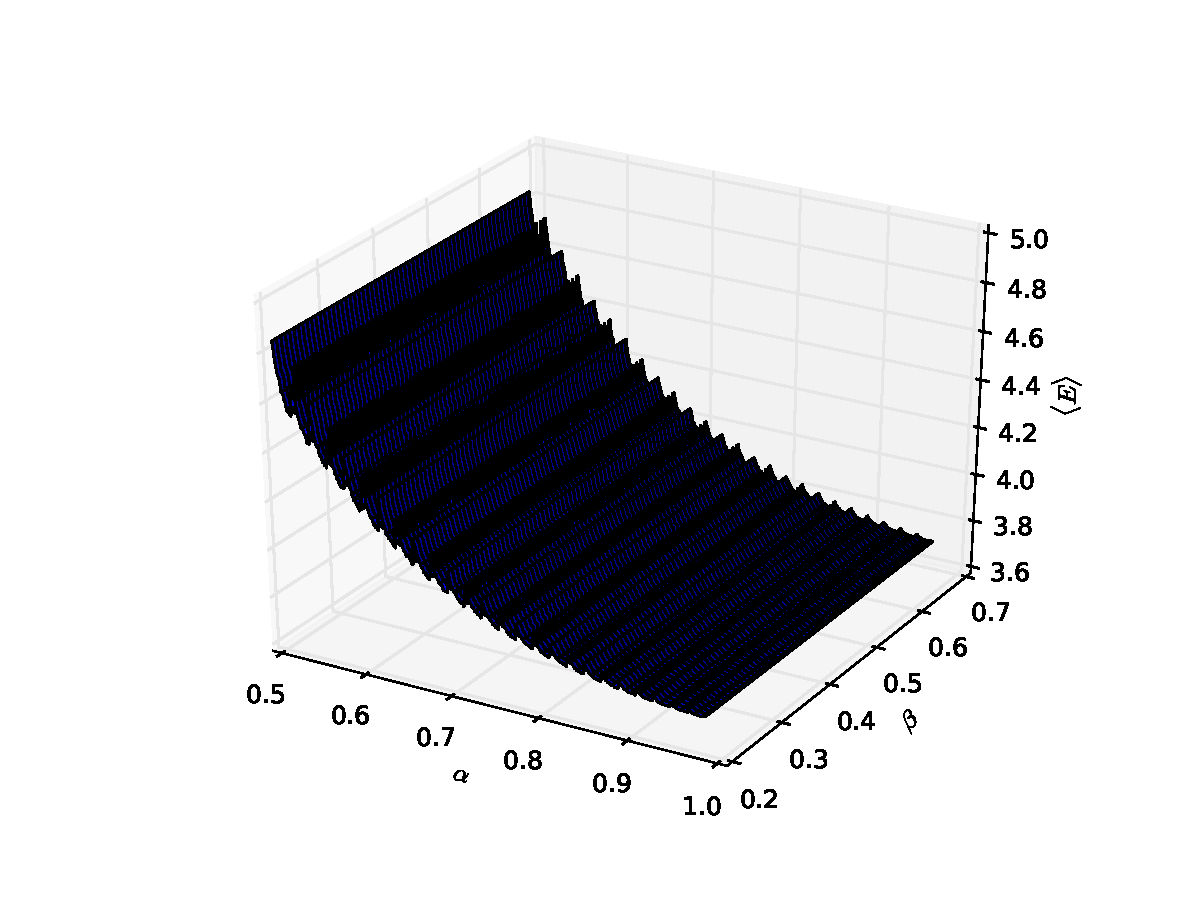
\includegraphics[width=\linewidth]{Plots/OptimalAlphaBeta_3DPlot.pdf}
\caption{3D plot of the energy expectation values as a function of $\alpha$ and $\beta$.}
\label{fig:3DPlot_AlphaBeta_Optimal}
\end{figure}

\FloatBarrier
\subsubsection{The Jastrow factor}
We are also interested on how important the correlations are when we introduce the Jastrow factor. Using the optimal variational parameter values, we can calculate the energy, variance as well as the mean distance for the wave function, with and without the Jastrow factor. Table \ref{table:Jastrow-Result} and \ref{table:Non-Jastrow-Result} shows the computed values, with and without the Jastrow factor respectively.

\begin{table}
\begin{center}
	\begin{tabular}{| l | l | l | l |}
	\hline
	 $\omega$ & Energy & Variance & Mean distance \\ \hline
	 0.01 & 0.0860071 & 0.000287508 & 24.8372 \\
	 0.5 & 1.99854 & 0.00217906 & 2.69878 \\
	 1 & 3.7269 & 0.0125113 & 1.81991 \\ \hline
	\end{tabular}
\caption{Computed energy, variance and mean distance for different frequencies with the Jastrow factor.}
\label{table:Jastrow-Result}
\end{center}
\end{table}

\begin{table}
\begin{center}
	\begin{tabular}{| l | l | l | l |}
	\hline
	 $\omega$ & Energy & Variance & Mean distance \\ \hline
	 0.01 & 0.0926694 & 0.00067256 & 21.94 \\
	 0.5 & 2.01448 & 0.00246614 & 2.36761 \\
	 1 & 3.75114 & 0.01486 & 1.67748 \\ \hline
	\end{tabular}
\caption{Computed energy, variance and mean distance for different frequencies without the Jastrow factor.}
\label{table:Non-Jastrow-Result}
\end{center}
\end{table}
We see from the tables that the energies, as well as the mean distance, is smaller once we introduce the Jastrow factor. The Jastrow factor serves as an attempt to give a lower energy ground state for our trial wave function. The advantage of this factor is that it only introduces one extra variational parameter. One could introduce many more variational parameters, and possibly obtain a lower energy ground state. However, too many variational parameters is not exactly ideal, as we would have too many free parameters to determine.

\FloatBarrier
\subsection{Testing the virial theorem}
We now want to test the virial theorem with the optimal values of $\alpha$ and $\beta$ that we found in the previous  task. The virial theorem states that the expectation of the total kinetic value is proportional to the expectation value of the total potential energy, i.e $\langle T \rangle \propto \langle V \rangle$. If we consider a pure harmonic oscillator potential, the virial theorem states
\begin{align*}
\langle T \rangle = \langle V \rangle
\end{align*}
We will use our optimal results of the variational parameters, for $\omega = 0.01$, $\omega = 0.5$ and $\omega=1$, to compute the expectation values of the kinetic and potential energy in the frequency range $\omega \in [0.01, 1]$. \footnote{I was not sure if the task was to calculate an optimal $\alpha$ and $\beta$ for every single frequency in this range or just use the optimal variational parameters to compute our results for $\omega \in [0.01, 1]$. I went ahead and did the latter, as calculating an optimal variational parameter for every frequency would take a lot of CPU time.}

Let us first consider the case where the electrons do not interact. In this case, we will have a pure harmonic oscillator system. Figure \ref{fig:Virial_NoCoulomb} shows the plot of $\langle T \rangle / \langle V \rangle$ as a function of $\omega$. We note that, for all different cases of optimal variational parameter, the ratio of the kinetic and potential energy is almost constant. However, since we have a pure harmonic oscillator, we would expect that $\langle T \rangle / \langle V \rangle = 1$, which is clearly not the case here. Exact reason for this is unknown, but the variational parameter could have played a big role here. It appears that the kinetic energy is a lot smaller than the potential energy, when $\alpha$ is smaller.
\begin{figure}[h]
\centering
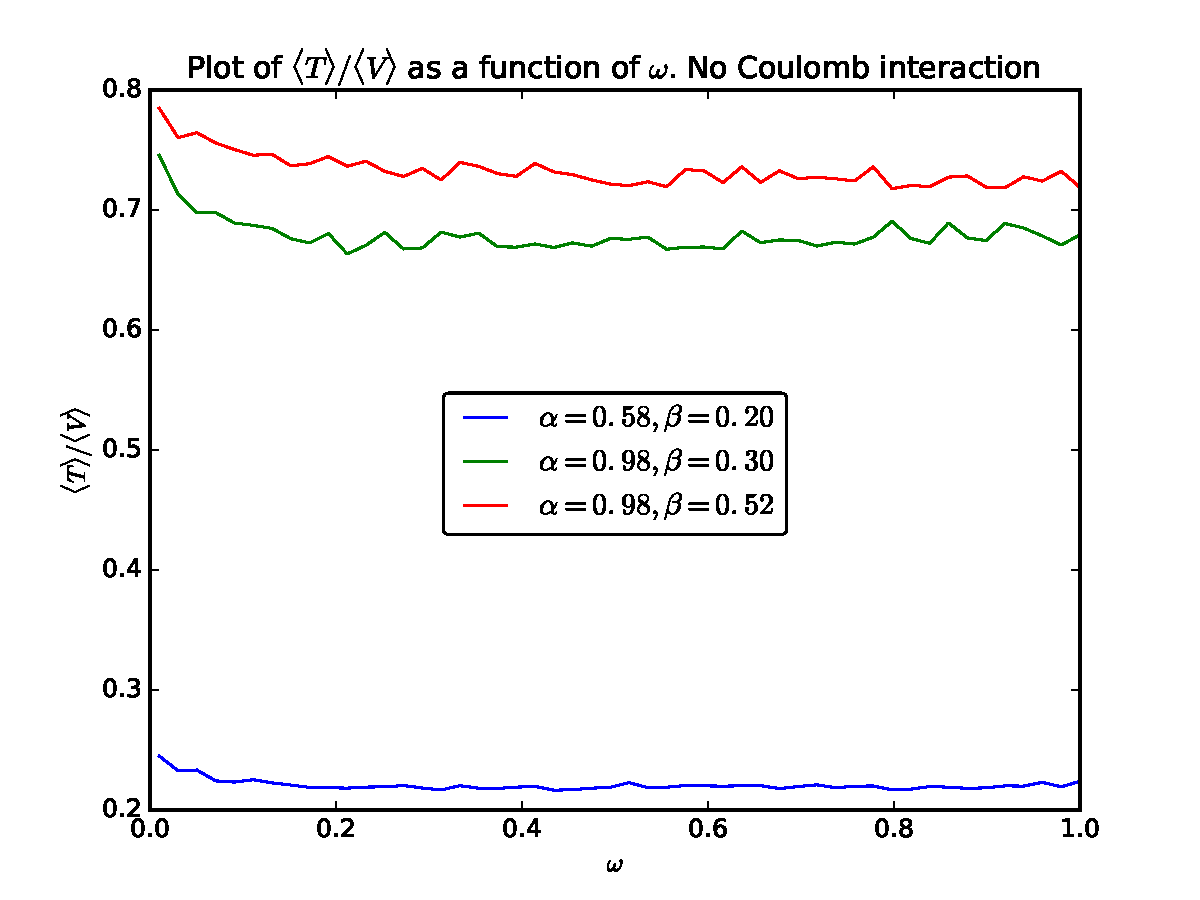
\includegraphics[width=\linewidth]{Plots/Virial_Plot_NoCoulombInt.pdf}
\caption{Plot of the ratio $\langle T \rangle / \langle V \rangle$ as a function of frequency $\omega$ with no Coulomb interaction.}
\label{fig:Virial_NoCoulomb}
\end{figure}


Let us now include Coulomb interaction between the electrons. A plot for this case can be found in figure \ref{fig:Virial_Plot}. We see here that the kinetic energy is larger for higher frequencies, and decreases as the frequency decreases. 

What this plot is telling us, is that the electrons have very small velocities (small kinetic energy) when the frequency is small. On top of that, when the frequency is smaller, the mean distance increases. What the plot shows is that the electrons, while being far away from each other, have very little movement. 

The harmonic oscillator potential is small when the frequency is smaller because $V(r) \propto \omega^2r^2$. When the potential is small, the electrons will roll 'slowly' down the potential well. This corresponds to the electrons having small kinetic energies. At the same time, the Coulomb force will push the electrons away from each other. The Coulomb force is stronger when the electrons are closer to each other, and weaker when they are further apart.

What this means, is that the electrons will never reach the bottom of the harmonic oscillator potential, due to the Coulomb force. However, the Coulomb force will not act on the electrons very strongly because they are so far away from each other. In other words, when $r_{12}$ is large, the Coulomb force will be small.

When the Coulomb force is weak and the electrons are slowly rolling down the potential well, the electrons will in the end not move a whole lot. The acceleration (or velocity) caused by the Coulomb force, and the acceleration that arises when the electrons are rolling down the potential, will sort of cancel each other out. Because of that, the electrons will not have a lot of movement, and is therefore bound to a very specific spot. An illustration of this can be found in figure \ref{fig:Virial_Example}. \footnote{Similar analogy was used in Project 2.}

\begin{figure}[h]
\centering
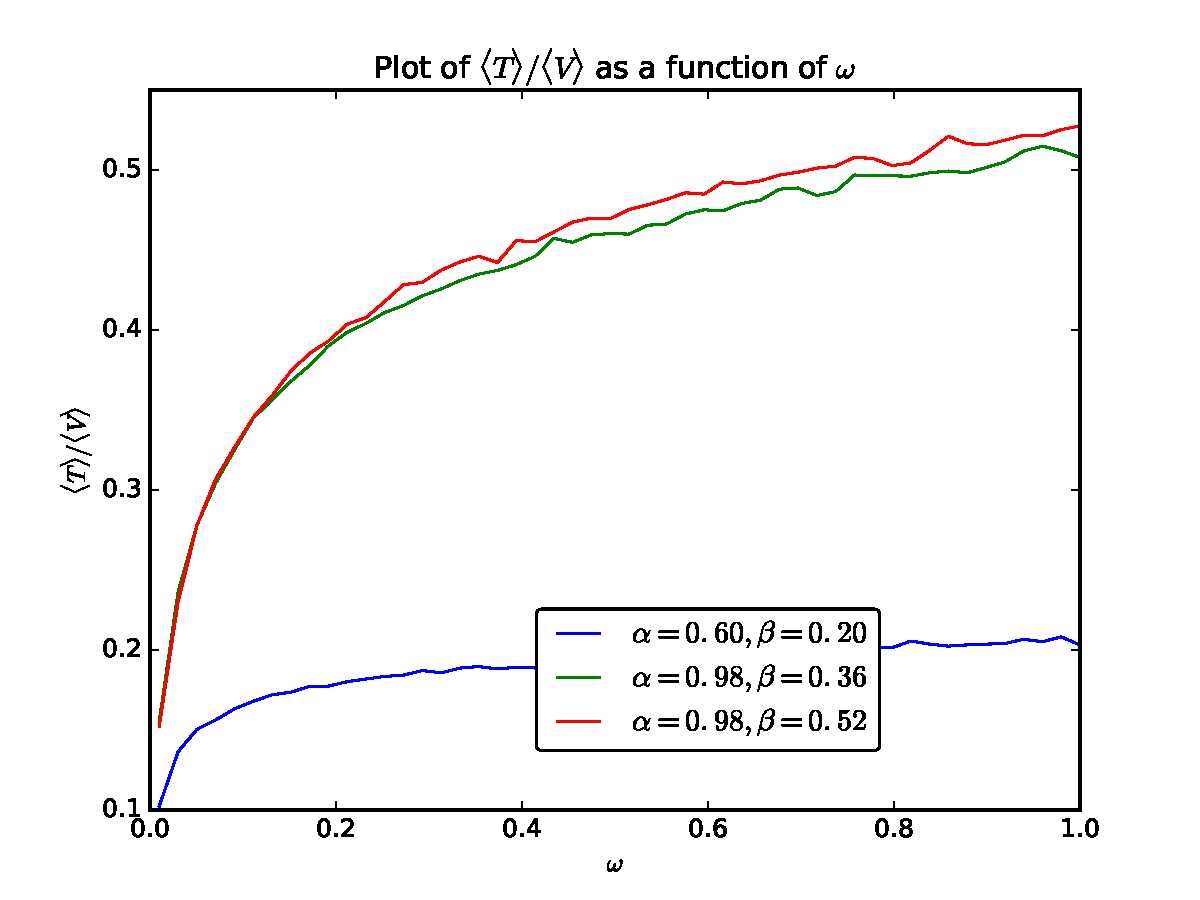
\includegraphics[width=\linewidth]{Plots/Virial_Plot.pdf}
\caption{Plot of the ratio $\langle T \rangle / \langle V \rangle$ as a function of frequency $\omega$ with Coulomb interaction.}
\label{fig:Virial_Plot}
\end{figure}


\begin{figure}[h]
\centering
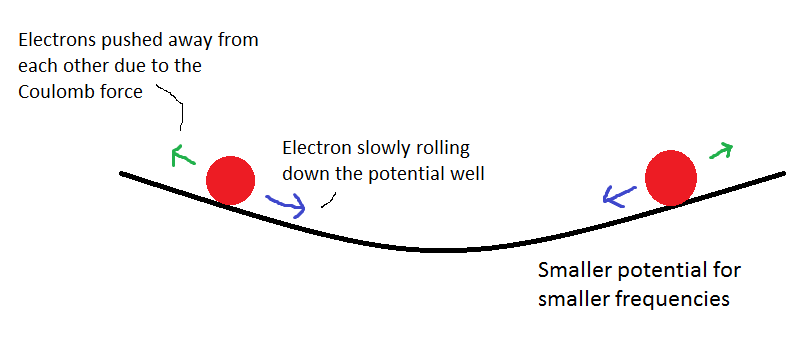
\includegraphics[width=\linewidth]{Virial-example.png}
\caption{Illustration of two electrons rolling down a small potential. The Coulomb pushes the electrons away from each other. However, the force will be very small because they are already far away from each other. The velocities from the Coulomb force will therefore 'cancel' out the velocity the electron is rolling down with.}
\label{fig:Virial_Example}
\end{figure}

Once again, we see that the kinetic energy is very small , with respect to the potential energy, when $\alpha$ is small. The variational parameter of $\alpha$ definitely plays a role to the kinetic energy, but the exact reasons is unknown to me.

Let us once again look at the stability of the Metropolis algorithm. In this example, we will plot the ratio $\langle T \rangle / \langle V \rangle$ with Coulomb interaction with $\alpha = 0.98$ and $\beta = 0.48$. An example of this can be found in figure \ref{fig:Stability_virial}. I have decided to cut out $N_{mc} = 100, 1000$ out of this plot as it cluttered the whole plot, thus making it harder to read. As we see from this figure, when we lower the number of Monte Carlo cycles, the results tend to 'jump' a little bit. That is, the algorithm is slightly less stable. Even though they are less stable, the results are still incredibly good.
\begin{figure}[h]
\centering
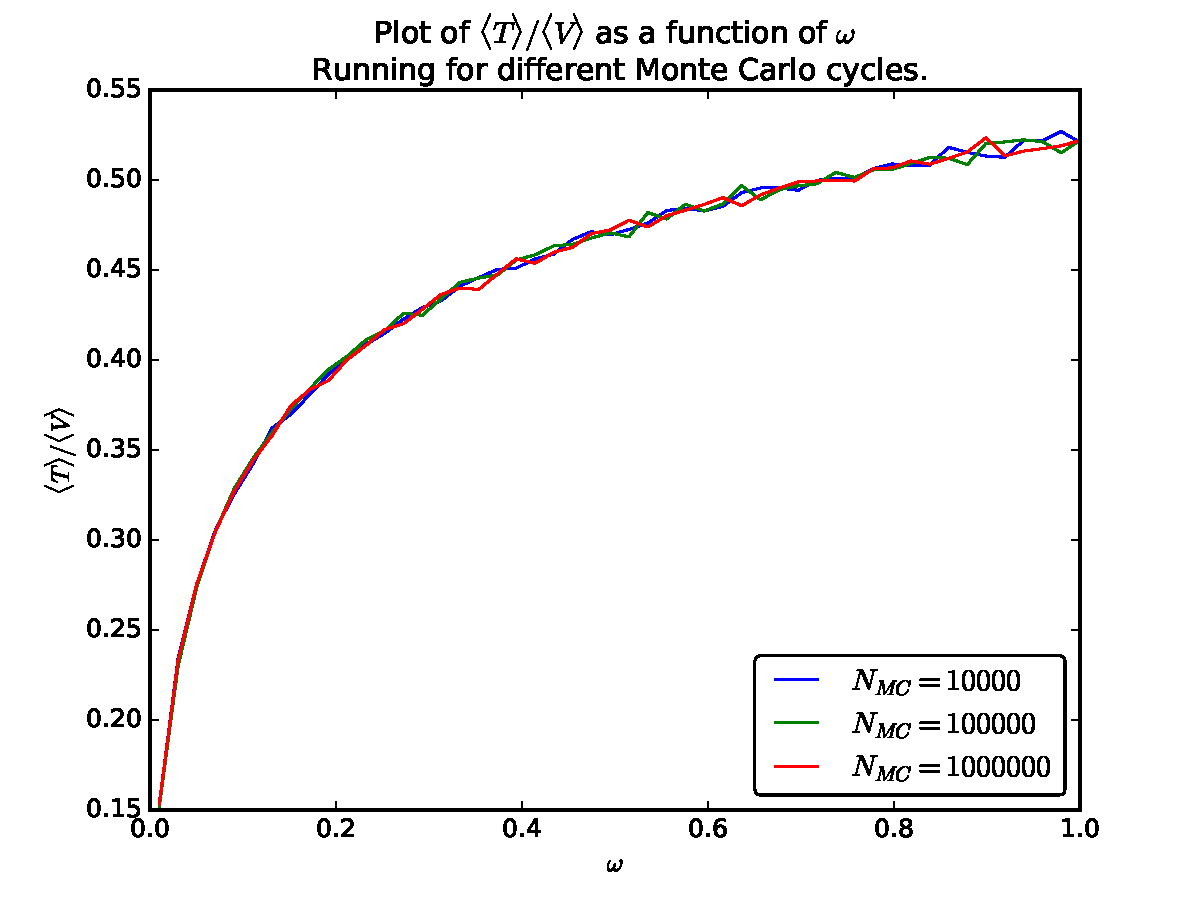
\includegraphics[width=\linewidth]{Plots/Virial_stability_test.pdf}
\caption{Stability test using the virial problem. Plot is using the case with $\alpha = 0.98$ and $\beta = 0.48$.}
\label{fig:Stability_virial}
\end{figure}
\FloatBarrier
\section{Conclusion}\label{section:conclusion}
From the results, we saw that using the Metropolis algorithm (a variational Monte Carlo method) to compute our harmonic oscillator system gave incredibly stable, and also fairly precise, results. If we look back to project 2, we used Jacobi's method to solve this system. The results back then were also very good, but the computation time for Jacobi's method was/is significantly longer than the Metropolis algorithm.

The physical results were fairly similar to project 2 as well. One example of this is the computed mean distance between the electrons. We knew that the electrons would be further apart when the frequency is smaller, and the results from this project agrees with what we observed in project 2. 

Of course, like any Monte Carlo method, increasing the number of Monte Carlo cycles could possibly give even more stable results, compared to what we obtained. However, we saw that, even with a lower number of Monte Carlo cycles, the results were incredibly stable.  
\FloatBarrier
\section{Appendix}
\begin{figure}[h]
\centering
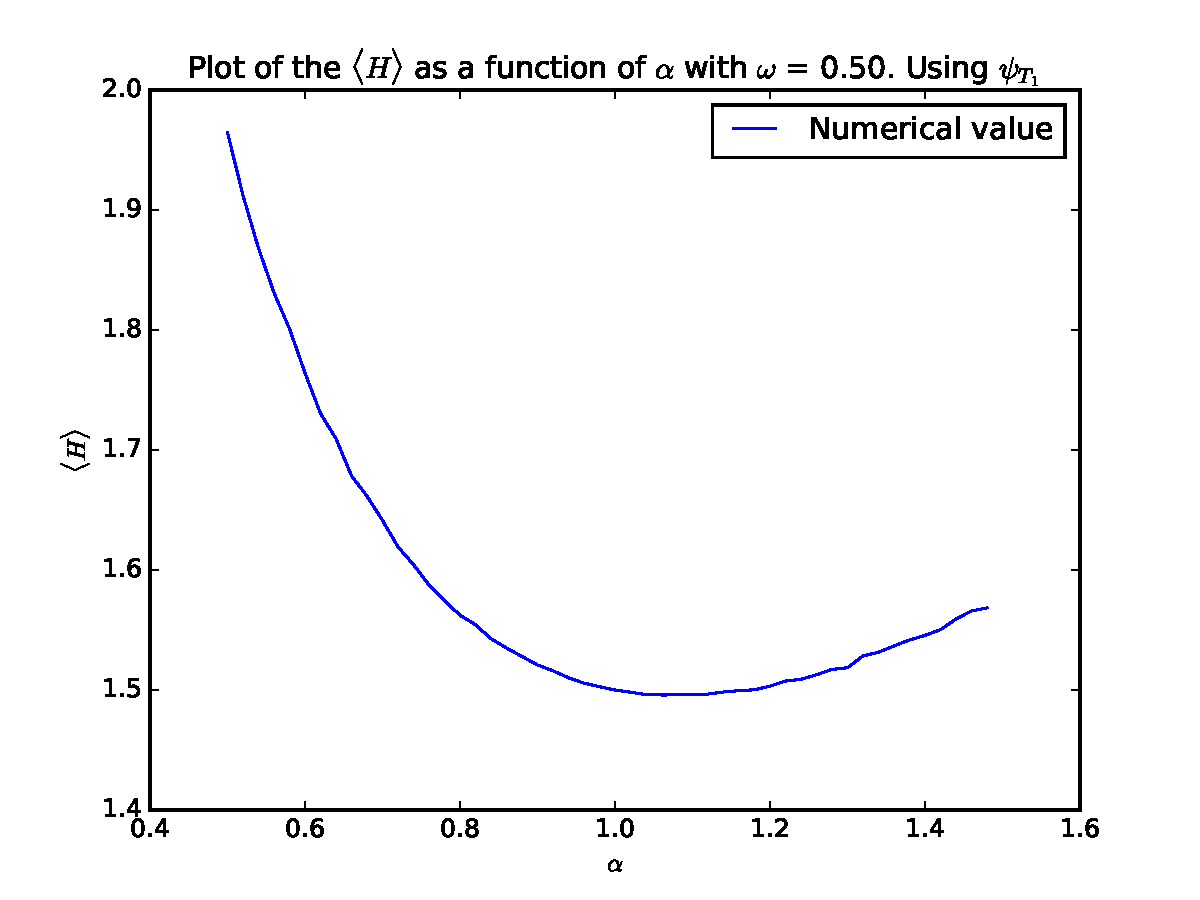
\includegraphics[width=\linewidth]{Plots/Energy_alpha_plot_omega05.pdf}
\caption{Plot of the Energy as a function of $\alpha$ with $\omega = 0.5$.}
\label{fig:Energy_alpha_omega05}

\end{figure}
\begin{figure}[h]
\centering
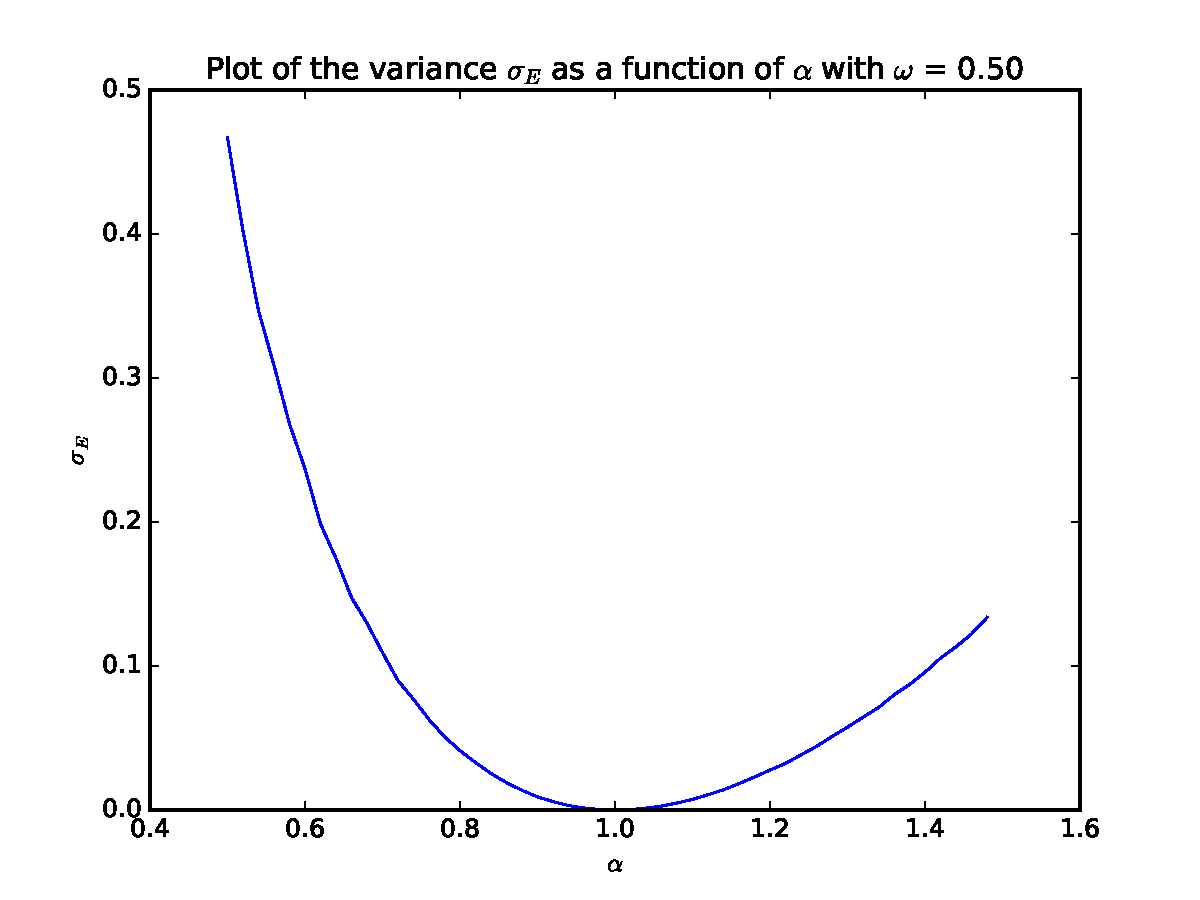
\includegraphics[width=\linewidth]{Plots/Variance_alpha_plot_omega05.pdf}
\caption{Plot of the variance as a function of $\alpha$ with $\omega = 0.5$.}
\label{fig:Variance_alpha_omega05}
\end{figure}

\begin{figure}[h]
\centering
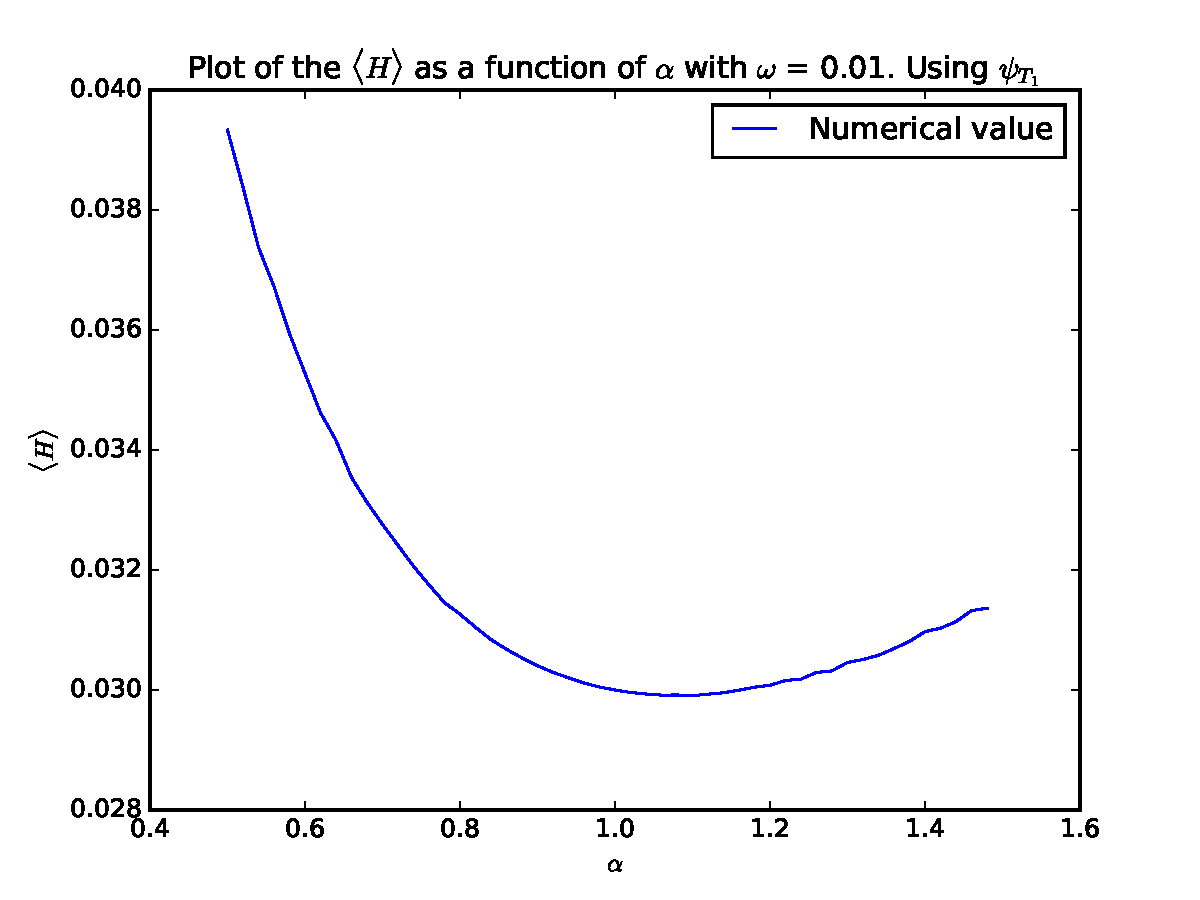
\includegraphics[width=\linewidth]{Plots/Energy_alpha_plot_omega001.pdf}
\caption{Plot of the Energy as a function of $\alpha$ with $\omega = 0.01$.}
\label{fig:Energy_alpha_omega001}
\end{figure}
\begin{figure}[h]
\centering
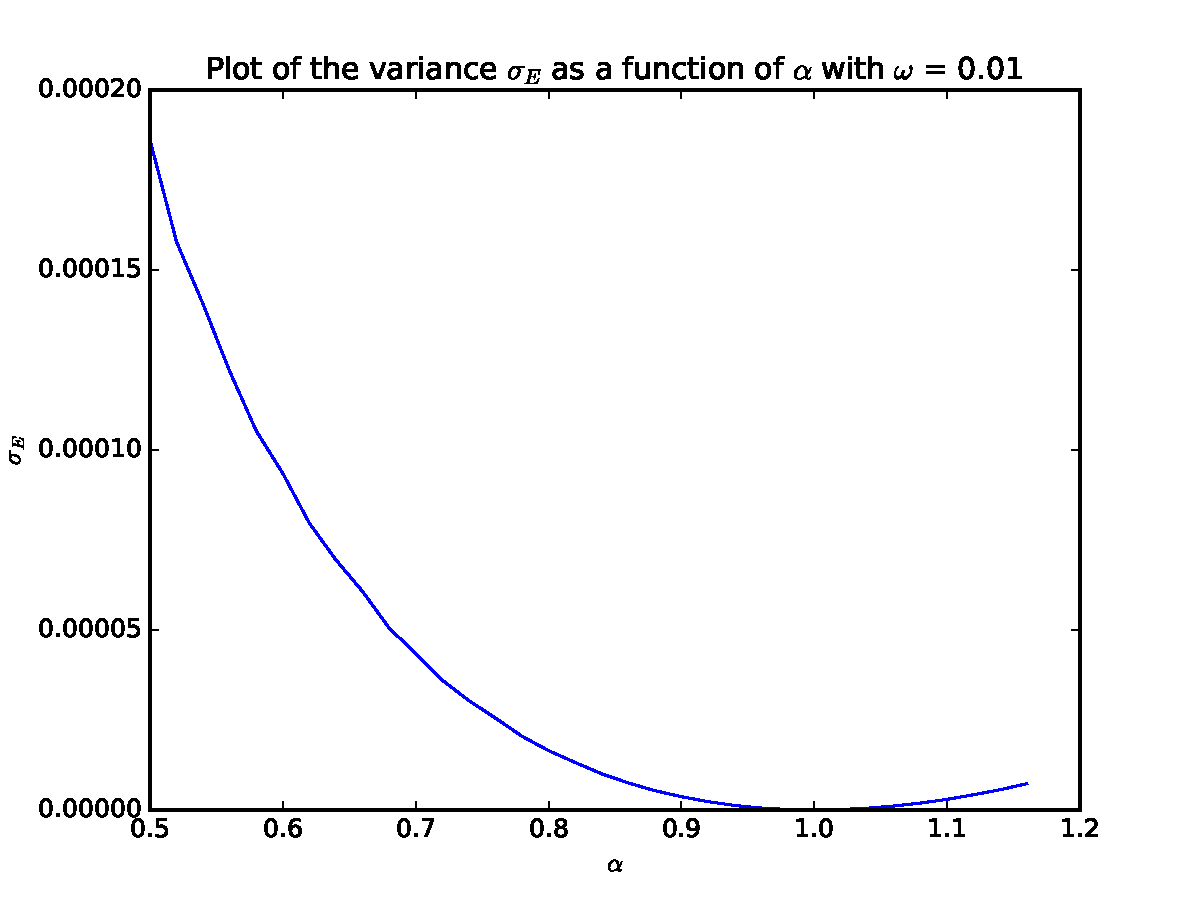
\includegraphics[width=\linewidth]{Plots/Variance_alpha_plot_omega001.pdf}
\caption{Plot of the variance as a function of $\alpha$ with $\omega = 0.01$.}
\label{fig:Variance_alpha_omega001}
\end{figure}


\FloatBarrier
\begin{thebibliography}{1}
    \bibitem{cpyhsics} M. Hjorth-Jensen, \emph{Computational Physics}, 2015, 551 pages
\end{thebibliography}
\end{document}